\documentclass{minimal}
\usepackage{graphicx,color}
\usepackage[papersize={576.00bp,432.00bp},text={576.00bp,432.00bp}]{geometry}
\begin{document}
\centering
% Title: glps_renderer figure
% Creator: GL2PS 1.3.8, (C) 1999-2012 C. Geuzaine
% For: Octave
% CreationDate: Fri Nov 10 18:01:37 2017
\setlength{\unitlength}{1pt}
\begin{picture}(0,0)
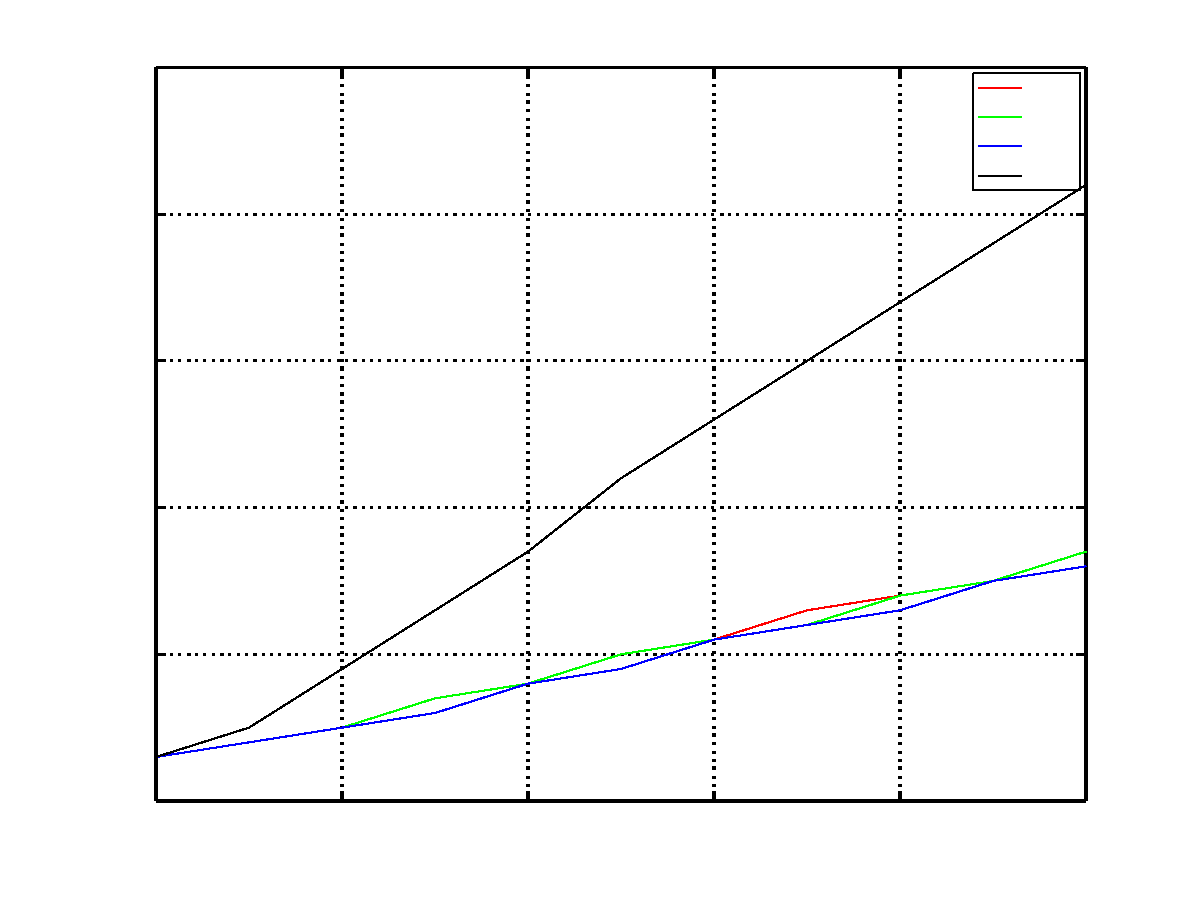
\includegraphics{current_brightness_1-inc}
\end{picture}%
\begin{picture}(576,432)(0,0)
\fontsize{12}{0}
\selectfont\put(74.88,42.5189){\makebox(0,0)[t]{\textcolor[rgb]{0,0,0}{{0}}}}
\fontsize{12}{0}
\selectfont\put(164.16,42.5189){\makebox(0,0)[t]{\textcolor[rgb]{0,0,0}{{20}}}}
\fontsize{12}{0}
\selectfont\put(253.44,42.5189){\makebox(0,0)[t]{\textcolor[rgb]{0,0,0}{{40}}}}
\fontsize{12}{0}
\selectfont\put(342.72,42.5189){\makebox(0,0)[t]{\textcolor[rgb]{0,0,0}{{60}}}}
\fontsize{12}{0}
\selectfont\put(432,42.5189){\makebox(0,0)[t]{\textcolor[rgb]{0,0,0}{{80}}}}
\fontsize{12}{0}
\selectfont\put(521.28,42.5189){\makebox(0,0)[t]{\textcolor[rgb]{0,0,0}{{100}}}}
\fontsize{12}{0}
\selectfont\put(69.8755,47.52){\makebox(0,0)[r]{\textcolor[rgb]{0,0,0}{{0}}}}
\fontsize{12}{0}
\selectfont\put(69.8755,117.936){\makebox(0,0)[r]{\textcolor[rgb]{0,0,0}{{10}}}}
\fontsize{12}{0}
\selectfont\put(69.8755,188.352){\makebox(0,0)[r]{\textcolor[rgb]{0,0,0}{{20}}}}
\fontsize{12}{0}
\selectfont\put(69.8755,258.768){\makebox(0,0)[r]{\textcolor[rgb]{0,0,0}{{30}}}}
\fontsize{12}{0}
\selectfont\put(69.8755,329.184){\makebox(0,0)[r]{\textcolor[rgb]{0,0,0}{{40}}}}
\fontsize{12}{0}
\selectfont\put(69.8755,399.6){\makebox(0,0)[r]{\textcolor[rgb]{0,0,0}{{50}}}}
\fontsize{10}{0}
\selectfont\put(298.08,28.5189){\makebox(0,0)[t]{\textcolor[rgb]{0,0,0}{{Brightness levels (\%)}}}}
\fontsize{10}{0}
\selectfont\put(49.8755,223.56){\rotatebox{90}{\makebox(0,0)[b]{\textcolor[rgb]{0,0,0}{{Current (mA)}}}}}
\fontsize{10}{0}
\selectfont\put(123.984,364.392){\makebox(0,0)[l]{\textcolor[rgb]{0,0,0}{{$F_{red}$(x) = 0.141818x+2.63636}}}}
\fontsize{10}{0}
\selectfont\put(123.984,336.226){\makebox(0,0)[l]{\textcolor[rgb]{0,0,0}{{$R_{red}^2$ = 0.995745}}}}
\fontsize{10}{0}
\selectfont\put(123.984,293.976){\makebox(0,0)[l]{\textcolor[rgb]{0,0,0}{{$F_{green}$(x) = 0.14x+2.63636}}}}
\fontsize{10}{0}
\selectfont\put(123.984,265.81){\makebox(0,0)[l]{\textcolor[rgb]{0,0,0}{{$R_{green}^2$ = 0.995634}}}}
\fontsize{10}{0}
\selectfont\put(123.984,223.56){\makebox(0,0)[l]{\textcolor[rgb]{0,0,0}{{$F_{blue}$(x) = 0.134545x+2.54545}}}}
\fontsize{10}{0}
\selectfont\put(123.984,195.394){\makebox(0,0)[l]{\textcolor[rgb]{0,0,0}{{$R_{blue}^2$ = 0.994732}}}}
\fontsize{10}{0}
\selectfont\put(493.16,389.824){\makebox(0,0)[l]{\textcolor[rgb]{0,0,0}{{R}}}}
\fontsize{10}{0}
\selectfont\put(493.16,375.764){\makebox(0,0)[l]{\textcolor[rgb]{0,0,0}{{G}}}}
\fontsize{10}{0}
\selectfont\put(493.16,361.704){\makebox(0,0)[l]{\textcolor[rgb]{0,0,0}{{B}}}}
\fontsize{10}{0}
\selectfont\put(493.16,347.644){\makebox(0,0)[l]{\textcolor[rgb]{0,0,0}{{RGB}}}}
\fontsize{10}{0}
\selectfont\put(298.08,409.6){\makebox(0,0)[b]{\textcolor[rgb]{0,0,0}{{Current drawn by one neopixel per colour brightness.}}}}
\end{picture}
\end{document}
